\documentclass[tikz]{standalone}
\usepackage{tikz-feynhand}
\usepackage{feynmf}
% bubble diagram
\begin{document}
% loop diagram
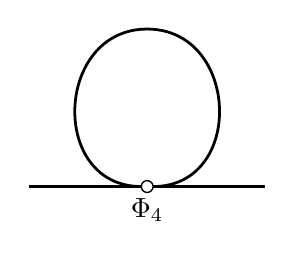
\begin{tikzpicture}
\begin{feynhand}
\vertex[ringdot] (a) at (0,0){};
\vertex (b) at (0,2); 
\vertex (c) at (1.5,0);\vertex (d) at (-1.5,0); % 両端
\propag[plain,line width = 1pt] (a) to (c);% 両端
\propag[plain,line width = 1pt] (d) to (a);% 両端
\propag[plain,line width = 1pt] (a) to [in=0, out=0, looseness=1.5] (b);
\propag[plain,line width = 1pt] (a) to [in=180, out=180, looseness=1.5] (b);
\node at (0,-0.3) {$\Phi_4$};
\end{feynhand}
\end{tikzpicture}
\end{document}
